\section{Implementering}
I følgende afsnit implementeres et elliptisk kurvekryptosystem til at udføre kryptering. Herefter vises et eksempel på en key-exchange, hvorefter sikkerheden i det implementerede system diskuteres.

\subsection{Valg af programmeringssprog}
Da kryptering er noget man gerne vil have sker hurtigst muligt, giver det bedst mening hvis det skal anvendes i industrien at bruge sprog såsom C eller C++. Jeg har dog valgt at lave mit program i python, da python understøtter heltal af arbitrær størrelse, hvilket C eller C++ ikke gør. Dette gør at koden bliver meget nemmere at skrive og forstå. 

\subsection{Valg af kurve}
Når vi skal lave en implementering i praksis, er det vigtigt at vælge en ”sikker” elliptisk kurve. Nogen kurver kan nemlig blive udsat for forskellige angreb, som det diskuteres mere i vurderingen af systemet. En af de mest kendte sider til at finde kurver på er safecurves.cr.yp.to, som laver store mængder forskning ifb. med forskellige typer af angreb på deres kurver inden de anbefales. Ud fra hjemmesiden vælger jeg kurven M-221, da den er verificeret som sikker (\cite{danielj.bernsteintanjalange2014}). Den har parametrene givet ved:
\begin{python}
# M-221 https://eprint.iacr.org/2013/647.pdf
p = 0x1FFFFFFFFFFFFFFFFFFFFFFFFFFFFFFFFFFFFFFFFFFFFFFFFFFFFFFD
A = 0x01c93a
B = 0x01
G = (0x04, 0x0f7acdd2a4939571d1cef14eca37c228e61dbff10707dc6c08c5056d)
n = 0x040000000000000000000000000015A08ED730E8A2F77F005042605B
\end{python}
Bemærk at talet er skrevet i hex, som det kan ses på præfiks givet ved $0x$

\subsection{Addition på elliptisk kurve}
For at kunne oversætte matematikken til kodning, skal vi ud fra vores endelige legeme fremstille en algoritme for additionsformlerne se definition. Hermed kan vi opskrive følgende (\cite{williamstein2006}):

\begin{algorithmic}

\If{$P_1 = \mathcal{O}$ or $P_2 = \mathcal{O}$} 
    \State \Return $P_3 = \mathcal{O}$
    \EndIf
\If{$x_1 = x_2 $ and $ y_1 = -y_2 $}
    \State \Return $P_3 = \mathcal{O}$
    \EndIf
\If{$P_1 = P_2$}
    \State $a \gets \frac{3x_{1}^2+A}{2\cdot y_{1}}$
\Else
    \State $\frac{y_{P}-y_{Q}}{x_{P}-x_{Q}}$
\EndIf
\State $x_3 \gets a^2 - x_1 - x_2$
\State $y_3 \gets -a(x_{3}- x_1 )- y_1$
\State \Return $(x_3, y_3)$

\end{algorithmic}

Da punktet $\mathcal{O}$ er et irrationelt tal, kan vi ikke regne med det på en computer. Vi definerer hermed \code{None} til at være lig med $O$ i koden. Bemærk også at ved division menes at tage den modulære multiplikative inverse som findes ved Euklids udvidede algoritme. Denne algoritme er implementeret via (\cite{andrewharrington}), hvorefter den er modificeret til \textit{kun} at returnere den modulære multiplikative inverse.

\subsection{Skalarmultiplikation}
\label{sec:skalarmultiplikation}
Vi opstiller nu pseudo-kode for algoritmen for skalarmultiplikation hvor n er antal gange til at addere og P er et punkt.
\\
\begin{algorithmic}
    \State def $mult(n, P)$

    \If{$n = n_E$}    \Comment{$n_E$ the order of the curve}
        \State \Return $\mathcal{O}$
    \ElsIf{$n < 0$}
        \State \Return $mult(-n, P)$ \Comment{run algorithm again with $-n$}
    \EndIf
    \State $new\_point \gets \mathcal{O}$
    \State $temp\_point \gets P$

    \While{$n$} \Comment{Continue until is false ($n=0$)}
        \If{$n \& 1 = true$} \Comment{Get first binary digit}
        \State $new\_point \gets new\_point + temp\_point$
        \EndIf
        \State $temp\_point \gets double(temp\_point)$ \Comment{same as P+P}
        \State $n \gets n>>1$ \Comment{Right shift binary number}
    \EndWhile
    \State \Return $new\_point$
\end{algorithmic}

Når der står \code{while n}, menes der at algoritmen vil fortsætte indtil det binære repræsentation for tallet n er lig med 0. Når der står at der foretages et right shift menes der at det tallet \code{1001} bliver til \code{100}, vi fjerner altså det første bit af tallet. 

\subsection{Hjælpefunktioner}
Udover at have addition og skalarmultiplikation er der en række andre hjælpefunktioner. Dette inkluderer bla. Andet \code{discriminant} som returnerer om ellipsen er valid for elliptisk kurvekryptografi. Funktionen \code{is\_on\_curve} returnerer \code{True} hvis punktet som er givet er på kurven, hvilket er smart til at tjekke udregninger. 

\subsection{Diffie-Hellmann key exchange eksempel}
For at lave et Diffie-Helmann key exchange bruger vi algoritmen som forklaret i \fref{tab:key_exchange_diffie}. Nedenunder ses et konkret eksempel på hvordan det laves. Først genererer Alice og Bob deres private og public keys. Bemærk \code{e} er et objekt for klassen \code{EllipticCurve} med \code{M-221}.
\begin{python}
# generate private keys
a = random.randint(1, p-1)
b = random.randint(1, p-1)

# generate public keys
A = e.mult(a, G)
B = e.mult(b, G)
\end{python}
Nu kan vi udregne deres shared secret:
\begin{python}
# Shared secret from other person public key
a_shared_secret = e.mult(a, B)
b_shared_secret = e.mult(b, A)

#check if keys are the same
assert a_shared_secret == b_shared_secret
print(a_shared_secret)
\end{python}
\code{> (E95FB24B62D35FDAE41997349B662AC4B71432A50408ADED7D5F21F, \\ 1F8A09D24045BF379EE29BFCC6D8A12271DED95E8691934F442ACFAA)}

Da begge deres secrets var den samme, kan vi konkludere at de har fået et \code{keypair} ved brug af hinandens \code{public\_keys}. I praksis anvender man kun $x$-koordinatet for ens secret, for at gemme mindre data.

\subsection{Sikkerheden i det implementerede system}
Som analyseret tidligere er krypteringen meget svær at bryde. Dog er der mange andre typer af angreb man kan lave. Problemet med et Diffie-Helmann key exchange er, at det kræver at man stoler på at den man kommunikerer med, ikke udgør sig for at være en anden. 
\begin{figure}[htbp]
    \centering
    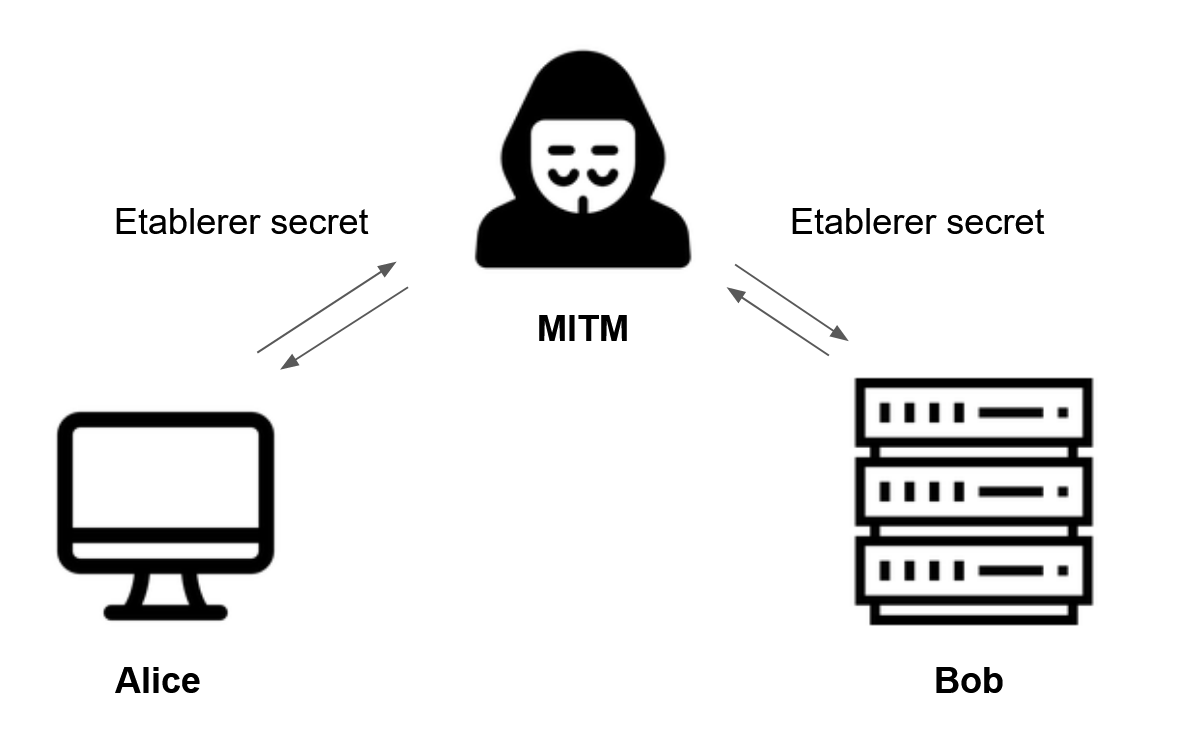
\includegraphics[width=0.6\linewidth]{images/MITM.png}
    \caption{MITM som udgiver sig for at være en anden}
    \label{fig:MITM}
\end{figure}
\FloatBarrier

Som det ses på \fref{fig:MITM}, kan MITM som oftest er en proxy udgive sig for at være en anden. Når Alice (computeren) sender en besked krypterer hun den med en public key som er en anden end den Bob har. MITM kan nu dekryptere beskeden og kryptere den igen med hans fælles secret med Bob (\cite{seanriley12017}). 

En måde at undgå et sådan angreb er ved at implementere en digital signatur som beviser at det er hende som har foretaget krypteringen. Bob kan hermed se at den secret key han modtager ikke kan være blevet ændret i. Eksempler på disse systemer er fx ECDSA (\cite{youssefelhousni2018}). 
Det kan hermed ses at sikkerheden i forhold til krypteringen er meget sikker i det implementerede system, men der er andre typer af angreb, som gør at systemet ikke kan anvendes i praktisk medmindre man er helt sikker på at ens kommunikation ikke er komprimeret. 
